\subsection{تولید شرح بر تصاویر با استفاده از روش‌های مبتنی بر نقطه توجه}
ایده‌ اصلی روش‌های مبتنی بر نقطه توجه از پژوهش‌های موجود در زمینه ترجمه ماشینی گرفته شده است. این دسته از پژوهش‌ها مدلی ارائه می‌دهند که با استفاده از آن بتوان هر کلمه از جملات تولیدی را با تمرکز بر یک یا بخشی از کلمات موجود در جمله مبدا‌، تولید کرد. به طور مشابه، در حوزه تولید خودکار شرح بر تصاویر، از این دسته از پژوهش‌ها به منظور حصول مدلی استفاده می‌شود که قادر باشد هر یک از کلمات موجود در جمله را با استفاده از بخشی از تصویر ورودی، تولید نماید.
\\
در این فصل، ابتدا ایده اصلی ترجمه مبتنی بر نقطه توجه را در حوزه ترجمه ماشینی ارائه خواهیم کرد و سپس کاربردهای این ایده را در حوزه تولید خودکار شرح بر تصاویر مورد بررسی قرار می‌دهیم. 

\subsection{روش‌های مبتنی بر نقطه توجه در حوزه ترجمه ماشینی}

همان‌طور که گفته شد، تمام روش‌های قبلی را می‌توان به دو مرحله زیر تقسیم کرد.
\begin{enumerate}
\item نگاشت نمونه‌ها از فضای تصاویر به فضای ویژگي‌ها
\item نگاشت نمونه‌ها از فضای ویژگی‌ها به فضای جملات
\end{enumerate}

در حوزه ترجمه ماشینی، به تابع نگاشت مرحله اول، انکودر\enfootnote{Encoder} و به تابع نگاشت مرحله دوم، دیکودر\enfootnote{Decoder} گفته می‌شود. در این بخش، ما از این عبارات برای ارجاع به مراحل اول و دوم الگوریتم استفاده می‌نماییم.
\\
چارچوب کاری انکودر-دیکودر، در تعداد زیادی از پژوهش‌های حوزه ترجمه ماشینی به عنوان چارچوب کاری اصلی مورد استفاده قرار گرفته است. تمام روش‌های قبلی که در فصول قبل ذکر شد نیز از همین چارچوب کاری به عنوان چارچوب اصلی بهره برده‌اند. به عنوان مثال در روش‌های مبتنی بر یادگیری عمیق برای تولید خودکار شرح بر تصاویر از شبکه‌های عصبی کانولوشنی به طور معمول به عنوان انکودر و از شبکه‌های عصبی بازگشتی به عنوان دیکودر استفاده می‌شود.
\\
شکل \ref{fig:5-1} نشان‌دهنده ساختار کلی چارچوب کاری انکودر-دیکودر است.

\begin{figure}[h]
\centering
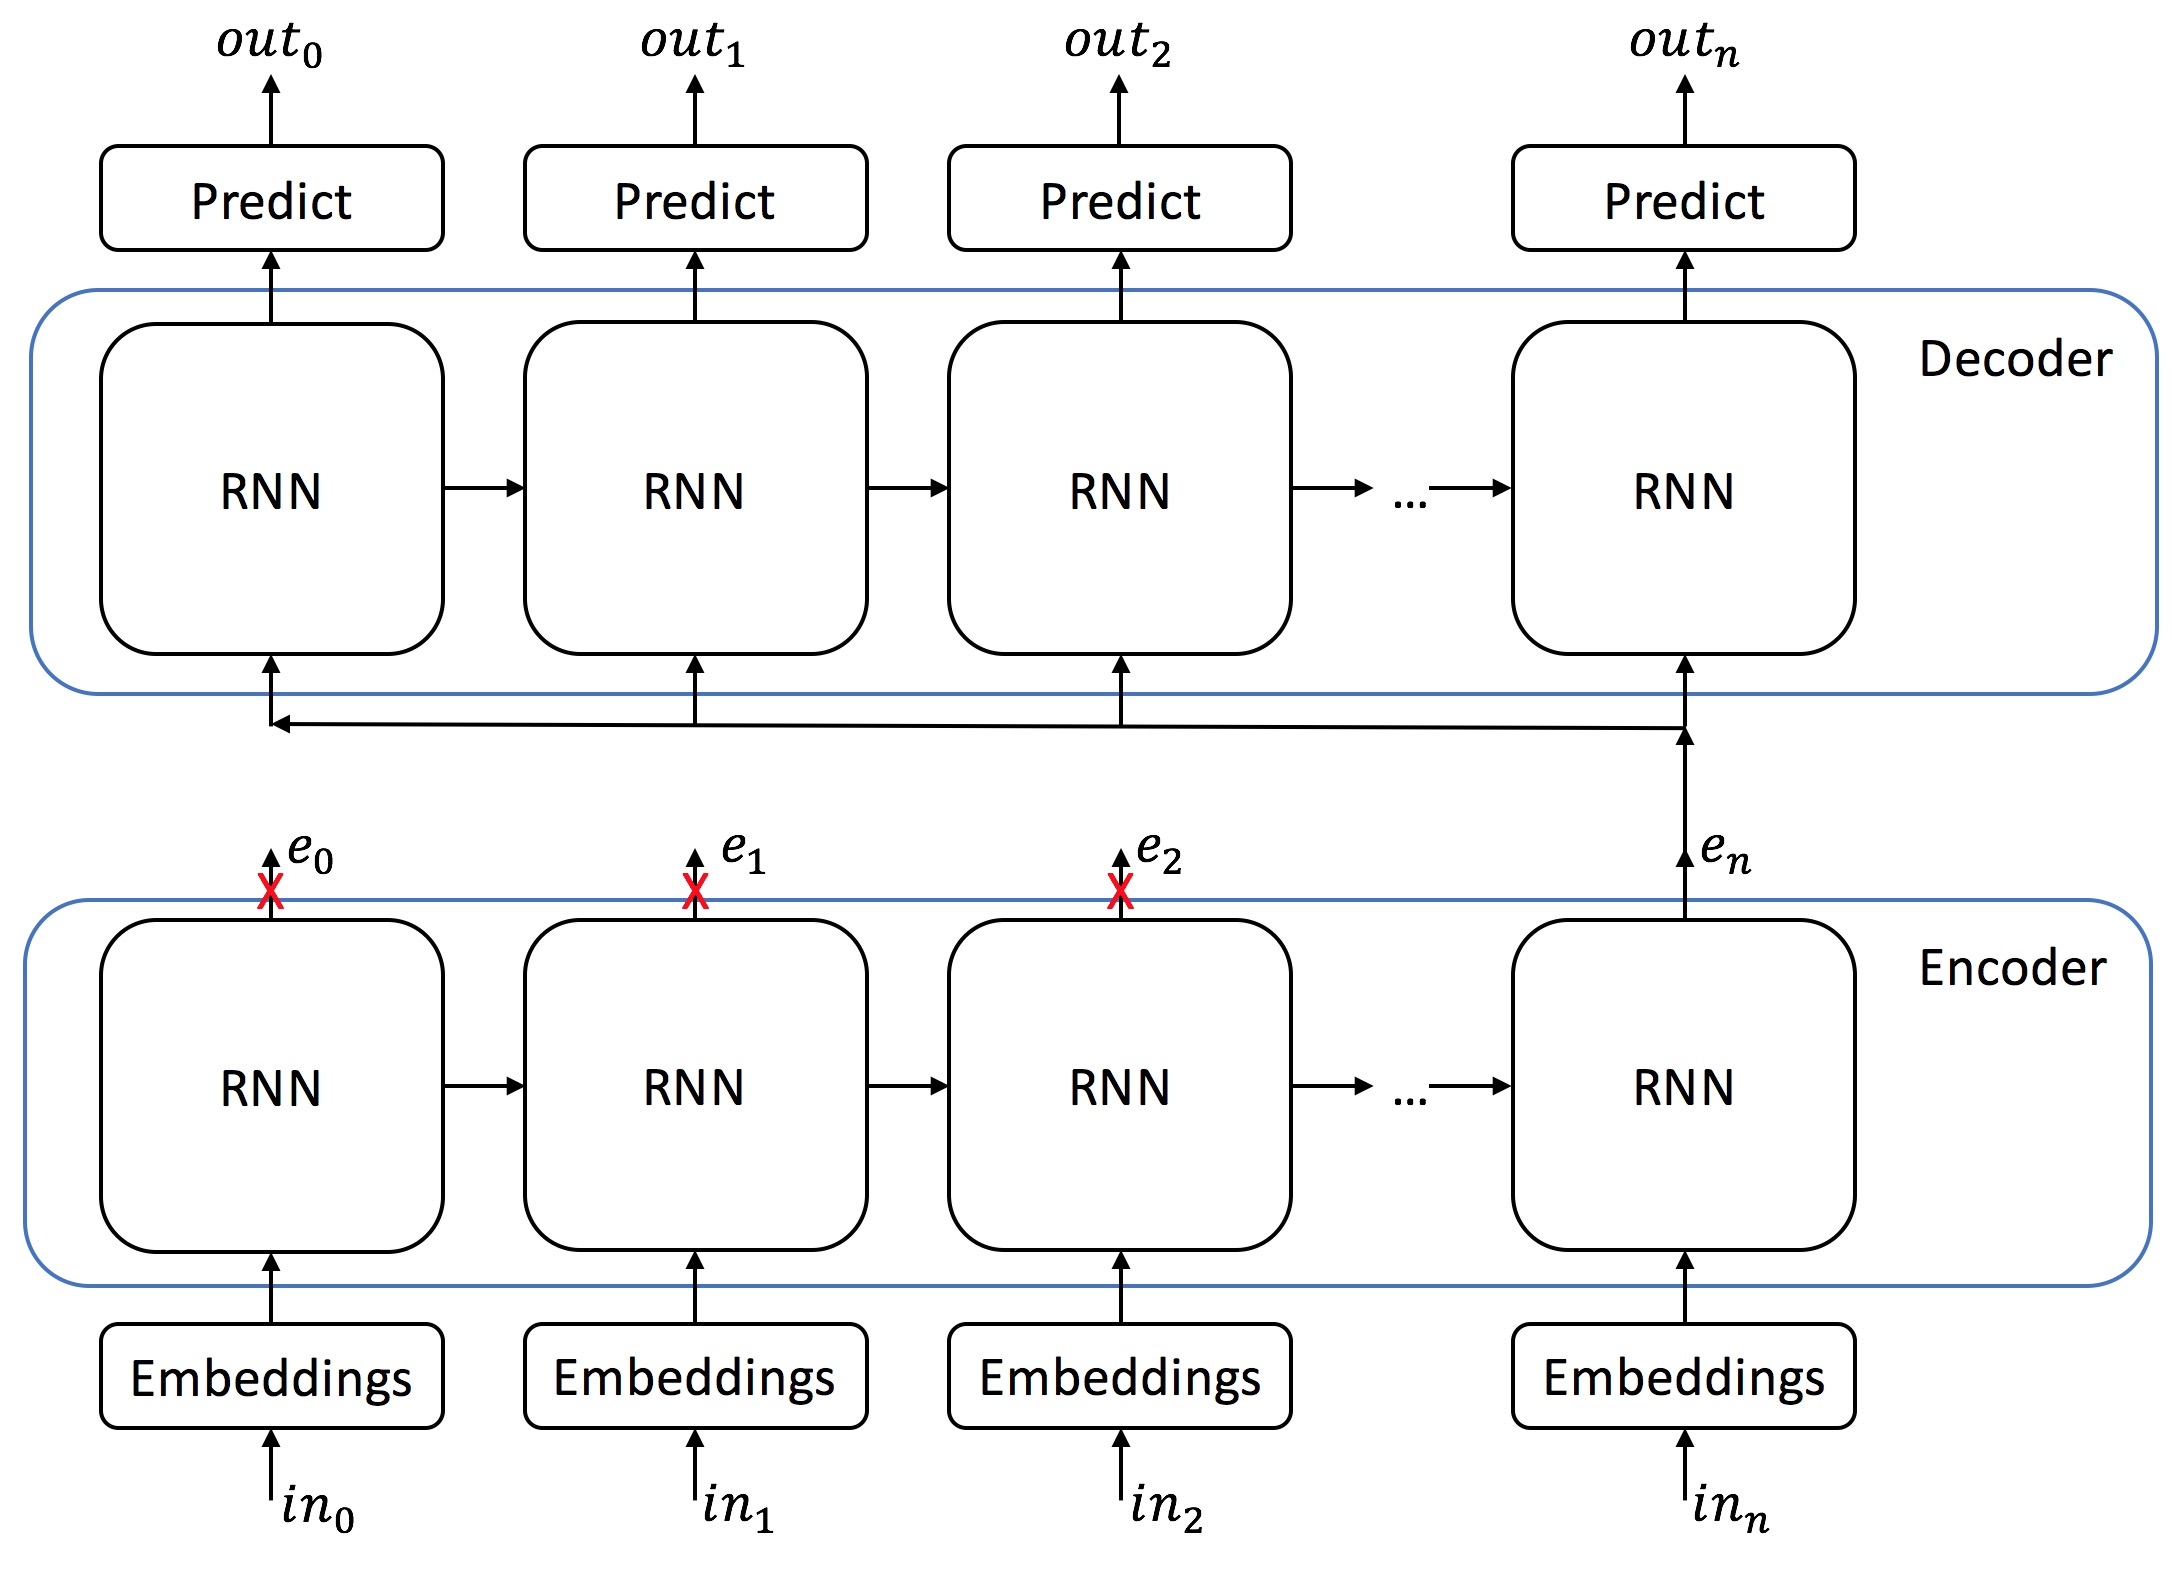
\includegraphics[scale=0.4]{Imgs/encoder-decoder.jpg}
\caption{ساختار کلی چارچوب کاری انکودر-دیکودر}
\label{ref:fig:5-1}
\end{figure}


در ادامه به بررسی بخش‌های مختلف این چارچوب کاری می‌پردازیم و سپس ایده اصلی روش‌های مبتنی بر نقطه توجه را که توسط آقای بنجیو در پژوهش \cite{bahdanau2014neural} در سال 2014 ارائه شده است، مورد بررسی قرار خواهیم 
داد.


\subsubsection{انکودر}
 انکودر در این چارچوب کاری، با گرفتن یک جمله به عنوان ورودی، بردار ویژگی متناظر جمله مبدا را تولید می‌کند. جمله ورودی با دنباله‌ای از کلمات مدل می‌شود. همین‌طور هر کلمه را با یک بردار $n$ بعدی، که $n$ تعداد کلمات موجود در دیکشنری است، مدل می‌شود. به این ترتیب، هر جمله ورودی، یک بردار با طول متغیر است که هر مولفه آن خودش برداری به ابعاد  $n$ است. از طرفی بردار خروجی، که همان بردار ویژگی‌ها است، یک بردار با طول ثابت و قراردادی خواهد بود.
 \\
 عموما در کاربردهای ترجمه ماشینی در هر دو بخش انکودر و دیکودر از شبکه‌های عصبی بازگشتی استفاده می‌شود. در شبکه‌های عصبی بازگشتی، خروجی هر مرحله تابعی از ورودی آن مرحله و حالت شبکه در مرحله جاری است. با فرض این‌که $h_t$ حالت شبکه در زمان $t$ را نمایش دهد می‌توان رابطه تولید خروجی توسط شبکه عصبی بازگشتی را مطابق با \eqref{eq:5-1} تعریف نمود.
\begin{align*}
h_t& = f(X_t , h_{t-1}) \\
C& = q(h_1, \cdots, h_L)
\numberthis 
\label{eq:5-1}
\end{align*}
به طور معمول از شبکه 
\lr{LSTM}
 به عنوان تابع $f$ استفاده می‌شود و همین‌طور به جای استفاده از تابع $q$ حالت نهایی شبکه به عنوان بردار ویژگی مورد استفاده قرار می‌گیرد
\cite{bahdanau2014neural}.

\subsubsection{دیکودر}

 دیکودر به منظور نگاشت فضای ویژگی‌ها به فضای جملات مورد استفاده قرار می‌گیرد. خروجی انکودر، ورودی دیکودر است. با این فرض، ورودی دیکودر یک بردار ویژگی با طول ثابت است و خروجی آن که یک جمله به زبان مقصد است، همانند جمله مبدا، یک بردار با طول متغیر شامل بردارهای بازنمایی کلمات است. دیکودر در اصل در هر مرحله، به دنبال یافتن کلمه‌ای است که با داشتن کلمات تولید شده قبلی و بردار ویژگی موجود، محتمل‌ترین کلمه نسبت به بقیه کلمات موجود در دیکشنری باشد. تابع احتمال مربوطه را می‌توان به فرم \eqref{eq:5-2} تعریف نمود.
 
 \begin{equation}
 p(y_t | C, y_1, y_2, \cdots, y_{t-1}) = g(y_t, s_t, C)
 \label{eq:5-2}
 \end{equation}

در رابطه \eqref{eq:5-2}، $C$ نشان‌دهنده بردار ویژگی‌، $y_i$ نشان‌دهنده لغت $i$ام تولید شده از زبان مقصد و بردار $s_t$ نشان‌دهنده حالت شبکه بازگشتی مورد استفاده به عنوان دیکودر است.


 شکل \ref{fig:decoder} ساختار کلی دیکودر را نمایش می‌دهد.

\begin{figure}[h]
\centering
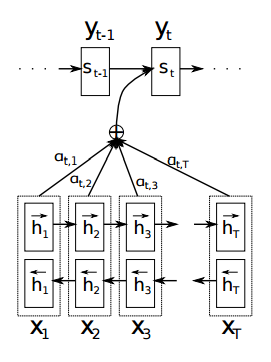
\includegraphics[scale=0.7]{Imgs/5-decoder.png}
\caption{ساختار دیکودر مورد استفاده در چارچوب کاری \cite{bahdanau2014neural}}
\label{fig:decoder}
\end{figure}

\subsubsection{ایده اصلی استفاده از نقطه توجه}

همان‌طور که بیان شد، در چارچوب کاری انکودر-دیکودر، ابتدا جمله ورودی که شامل تعداد نامعلوم کلمه است به یک بردار با طول متغیر مدل می‌شود. بردار تولید شده توسط یک انکودر به یک بردار با طول ثابت، که همان بردار ویژگی‌ها است، نگاشت شده و در نهایت بردار ویژگی تولید شده توسط یک انکودر به یک بردار با طول متغیر که نماینده جمله زبان مقصد است، نگاشت می‌شود.
\\
فرآیند مذکور یک محدودیت جدی دارد و آن این است که انکودر باید بتواند تمام اطلاعات مورد نیاز برای تولید جمله را در یک بردار با طول ثابت بگنجاند و دیکودر باید بتواند تمام اطلاعات مورد نیاز خود را از همین بردار با موجود با طول ثابت، استخراج کند. این محدودیت باعث می‌شود قدرت کد کردن اطلاعات در بردار ویژگی کاهش یابد. برای حل این مشکل از ایده نقاط توجه استفاده می‌نماییم.
\\
در این دسته از روش‌ها به جای این‌که انکودر فقط یک بردار ویژگی تولید کند، بردارهای ویژگی مختلفی ایجاد می‌کند که هر بردار با تمرکز بر روی یک یا بخشی از جمله مبدا تولید شده است. به این ترتیب، هر بردار تولید شده شامل اطلاعات معنایی یک یا بخشی از جمله مبدا می‌باشد. به این طریق، دیکودر می‌تواند با انتخاب بین بردارهای معنایی تولید شده در هر مرحله، کلمه تولیدی را با تمرکز بر روی معنای یک کلمه و کلمات مجاور آن در جمله مبدا، تولید کند.
\\
در ادامه به بررسی تغییراتی که باید در انکودر و دیکودر اتفاق بیفتد تا بتوان به جای یک بردار ویژگی مجموعه‌ای از بردارهای ویژگی با تمرکز محلی ایجاد نمود و از آن‌ها برای تولید جمله استفاده نمود را مورد بررسی قرار می‌دهیم. برای سهولت فهم تغییرات، ابتدا تغییرات دیکودر را مطرح نموده و سپس به بررسی تغییرات انکودر خواهیم پرداخت.
\subsubsection{دیکودر در روش مبتنی بر نقطه توجه}
فرض می‌کنیم به جای تنها یک بردار ویژگی، $L$ بردار ویژگی از ورودی استخراج شده باشد. آن‌ها را در یک ماتریس به شکل $C = [c_1, \cdots, c_L]^T$ بازنمایی می‌نماییم. فرض می‌کنیم بردار ویژگی $c_i$ به دنباله حاشیه‌نویسی‌های\enfootnote{Annotation} $h = [h_1, \cdots, h_L]^T$ وابسته است. حاشیه‌نویسی $h_i$ خود یک متغیر تصادفی به شکل برداری است که دارای دو ویژگی بسیار مهم می‌باشد.
\begin{enumerate}
\item .حاوی اطلاعات استخراج شده از تمام جمله است
\item تمرکز استخراج اطلاعات بر روی کلمه $i$ام و کلمات اطراف آن بوده است.
\end{enumerate}
با تعریف این دو ویژگی، حاشیه‌نویسی‌ها را می‌توان همان بردار ویژگی جمله تصور کرد با این شرط که علاوه بر این که معنای کل جمله را کد کرده‌اند، تمرکز بیشتری بر معنای کلمه $i$ام و کلمات مجاور آن دارند. به عبارت بهتر هر حاشیه‌نویسی علاوه بر این‌که معنای کلی جمله را کد می‌کند، حاوی معنای محلی مربوط به کلمات هم هست.
\\
با تعریف حاشیه‌نویسی به شکل فوق و با تکیه بر فرض‌های انجام شده، می‌توانیم مدل احتمالاتی ارائه شده را به شکل  \eqref{eq:5-3} تغییر دهیم. 
\begin{equation}
p(y_i| y_1, \cdots, y_{i-1}, X) = g(y_{i-1}, S_i, c_i)
\label{eq:5-3} 
\end{equation}
که در آن:
\begin{align*}
c_i = \Sigma_{j=1}^L \alpha_{ij}h_j
\numberthis
\label{eq:5-4}
\\
\alpha_{ij} = \frac{exp(e_{ij})}{\Sigma_{k=1}^Lexp(e_{ik})}
\numberthis
\label{eq:5-5}
\\
e_{ij} = f(s_{i-1}, h_j)
\numberthis
\label{eq:5-6}
\end{align*}

متغیر تصادفی $e_{ij}$ که در رابطه \eqref{eq:5-6} تعریف شده است نمایان‌گر میزان شباهت کلمه $i$ام در جمله خروجی به کلمه $j$ام در جمله ورودی است. وظیفه‌ این متغیر، هم‌ترازسازی\enfootnote{Alignment} ورودی و خروجی است. $\alpha_{ij}$ یک نرمال‌سازی روی امتیازهای محاسبه شده انجام می‌دهد. از این متغیر نرمال شده به عنوان وزن حاشیه‌نویسی‌ها استفاده می‌شود. مطابق با رابطه \eqref{eq:5-4} بردار ویژگی مورد استفاده برای تولید کلمه در جمله مقصد، از طریق یک میانگین‌گیری بر اساس وزن معنایی کلمات تولید می‌شود.
\\
در رابطه \eqref{eq:5-6} $s_{i-1}$ بردار حالت شبکه دیکودر در زمان $i-1$ و $f$ یک تابع امتیاز است. تابع امتیاز مورد استفاده در این رابطه را می‌توان با یک شبکه عصبی پیش‌رو\enfootnote{Feed Forward Neural Network} مدل‌سازی کرد. در صورت استفاده از شبکه عصبی پیش‌رو برای مدل‌سازی تابع شباهت، در صورتی که از هم‌ترازسازی نرم\enfootnote{Soft Alignment} استفاده شود، تابع هدف مشتق‌پذیر شده و می‌توانیم از الگوریتم پس‌انتشار خطا برای آموزش استفاده نماییم.


\subsubsection{انکودر در روش مبتنی بر نقطه توجه}
برای طراحی انکودر در این بخش، باید مکانیزمی ارائه شود که قادر باشد حاشیه‌نویسی‌های $h_1$ تا $h_L$ را طوری تولید کند که دو شرط مطرح شده در بخش قبلی را ارضا نمایند. به عبارت دیگر باید بردارهای ویژگی‌ای استخراج نماییم که علاوه بر این‌که حاوی معنای کل جمله باشند، هر یک از آن‌ها بر روی معنای یک کلمه و کلمات اطراف آن تمرکز بیشتری نسبت به سایر بردارها داشته باشند تا بتوانیم علاوه بر مدل‌سازی معنای کلی جمله، از معنای محلی کلمات هم استفاده نماییم.
\\
به این منظور از یک شبکه عصبی بازگشتی دوطرفه در مدل‌سازی انکودر استفاده می‌نماییم. شکل \ref{fig:biencoder} ساختار کلی یک شبکه عصبی بازگشتی دوطرفه را نمایش می‌دهد. 

\begin{figure}[h]
\centering
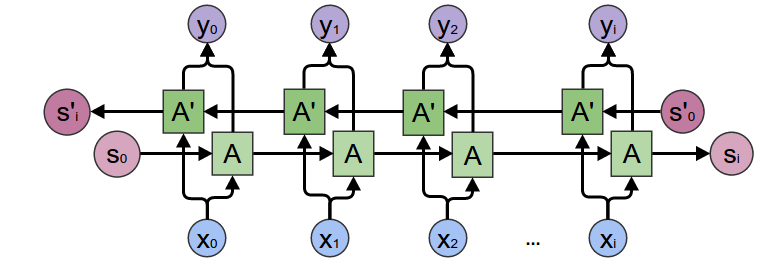
\includegraphics[scale=0.6]{Imgs/biencoder.png}
\caption{ساختار کلی یک شبکه عصبی بازگشتی دوطرفه}
\label{fig:biencoder}
\end{figure}

همان‌طور که در شکل \ref{fig:biencoder} مشخص است، یک شبکه عصبی بازگشتی دوطرفه شامل دو شبکه پیش‌رو در خلاف جهت یک‌دیگر است. حالت‌های مخفی شبکه پیش‌رو رو به راست را با $h_i^\rightarrow$ و حالت‌های مخفی شبکه پیش‌رو رو به چپ را با $h_i^\leftarrow$ نمایش می‌دهیم. همان‌طور که در شکل پیداست، خروجی‌های شبکه در این ساختار هم به حالت‌های سمت راست و کلمات سمت راست در جمله و هم به حالات و کلمات سمت چپ وابسته هستند. پس همین خروجی‌ها را می‌توان به عنوان حاشیه‌نویسی‌هایی که هر دو ویژگی را دارند مورد استفاده قرار داد.
	یکی از راه‌های ساده برای ایجاد حاشیه‌نویسی با استفاده از حالات شبکه‌های پیش‌رو رو به راست و رو به چپ این است که مطابق با رابطه \eqref{eq:5-7} با پشت سر هم قرار دادن حالات شبکه، حاشیه‌نویسی مورد نیاز را تولید نماییم.
	\begin{equation}
	h_j = [{h_j^\rightarrow}^T, {h_j^\leftarrow}^T]^T
	\label{eq:5-7}
	\end{equation}



\subsection{روش‌های مبتنی بر نقطه توجه در حوزه تولید شرح متناظر تصویر}
در بخش قبل به بیان ایده اصلی روش‌های مبتنی بر نقطه توجه در حوزه ترجمه ماشینی پرداختیم. ساختار کلی انکودرها و دیکودرها در این قالب و همین‌طور نحوه تولید بردارهای ویژگی مختلف از جمله مبدا و استفاده از این بردارها در تولید جمله مقصد را مورد بررسی قرار دادیم. در این بخش  به بررسی پژوهش‌هایی خواهیم پرداخت که از این ایده در حوزه تولید شرح متناظر تصویر بهره‌ جسته‌اند.
\\
یکی از برجسته‌ترین و مورد توجه‌ترین پژوهش‌ها از این دست، پژوهشی است که آقای بنجیو و همکارانش در سال 2015 ارائه داده‌اند
\cite{xu2015show}.
در این بخش به بررسی این پژوهش خواهیم پرداخت.

\subsubsection[تولید شرح متناظر تصویر با استفاده از توجه بصری و شبکه‌های عصبی]{تولید شرح متناظر تصویر با استفاده از توجه بصری و شبکه‌های عصبی \cite{xu2015show}}
	
در این پژوهش که در سال 2015 توسط آقای بنجیو و همکارانش ارائه شده است از ایده استفاده از توجه در حوزه ترجمه ماشینی استفاده شده است تا شرح متناظر تصاویر با دقت بیشتری تولید شود. چارچوب کاری انکودر-دیکودر مانند آن‌چه در بخش قبلی مطرح شد در این پژوهش مورد استفاده قرار گرفته است.
\\
انکودر ارائه شده در این پژوهش، یک شبکه عصبی کانولوشنی است که قادر به تولید $L$ بردار ویژگی مختلف است. به هر یک از این بردارهای ویژگی یک حاشیه‌نویسی\enfootnote{Annotation} تصویر گفته می‌شود. بردارهای حاشیه‌نویسی، همان‌طور که در بخش قبل ذکر شد، باید دارای دو شرط زیر باشند:
\begin{enumerate}
\item حاوی معنای تصویر به طور کلی باشند.
\item تمرکز بیشتری روی یکی از بخش‌های تصویر داشته باشند.
\end{enumerate}
برای این‌که بتوانیم دو شرط فوق را در بردارهای حاشیه‌نویسی تولید شده از انکودر بگنجانیم از خروجی لایه ما قبل آخر شبکه عصبی کانولوشنی به عنوان بردارهای حاشیه‌نویسی استفاده می‌کنیم. هر بردار حاشیه‌نویسی یک بردار $D$ بعدی است که مربوط به یک بخش از تصویر می‌شود و آن را با $a_i$ نمایش می‌دهیم. بنابر این داریم:
\begin{equation}
a = \{a_1, a_2, \cdots, a_L\}, a_i \in R^D
\end{equation}

در این پژوهش از یک شبکه حافظه کوتاه‌مدت بلند به عنوان دیکودر استفاده شده است. این شبکه با دریافت مجموعه بردارهای حاشیه‌نویسی $a$، جمله‌ای به زبان انگلیسی تولید می‌کند که شامل دنباله‌ای از $C$ کلمه است. هر کلمه با یک بردار $K$ بعدی نمایش داده می‌شود که $K$ تعداد کلمات موجود در دیکشنری است. در هر یک از بردارهای بازنمایی کلمات فقط یک مولفه یک است و مابقی مولفه‌ها صفر هستند. مولفه‌ای که برابر با یک است نمایش‌دهنده اندیس کلمه در دیکشنری است.
\\
شکل \ref{fig:satenc} یک سلول از شبکه حافظه کوتاه‌مدت بلند مورد استفاده در این پژوهش به عنوان دیکودر را نمایش می‌دهد. 
\begin{figure}[h]
\centering
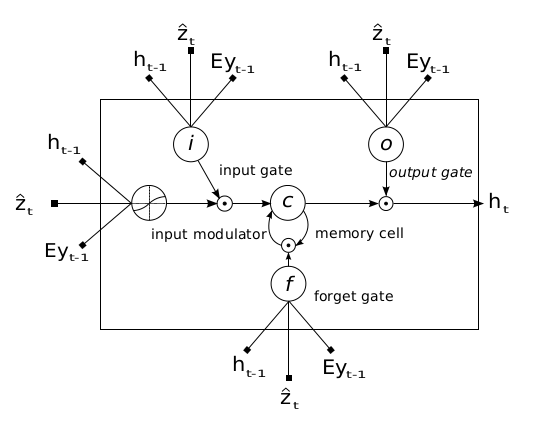
\includegraphics[scale=0.6]{Imgs/satenc.png}
\caption{یک واحد از شبکه حافظه کوتاه‌مدت بلند مورد استفاده در دیکودر پژوهش \cite{xu2015show}}
\label{fig:satenc}
\end{figure}
روابط مربوط به یادگیری این شبکه را می‌توان مطابق با روابط \eqref{eq:5-8} تا \ref{eq:5-13}  نمایش داد. در همه روابط، تابع $T$ یک تابع نگاشت خطی به شکل $T: R^{D+m+n}*R^n$ است که پارامترهای آن آموزش داده‌ شده‌اند. متغیر $i_t$ ورودی، $f_t$ خروجی سلول فراموشی، $c_t$ حافظه، $o_t$ خروجی و $h_t$ حالت مخفی شبکه را نمایش می‌دهند. 
\begin{align*}
i_t &= \sigma(T(Ey_{t-1}, h_{t-1}, \hat{z}_{t-1})) \numberthis \label{eq:5-8} \\
f_t &= \sigma(T(Ey_{t-1}, h_{t-1}, \hat{z}_{t-1})) \numberthis \label{eq:5-9} \\
o_t &= \sigma(T(Ey_{t-1}, h_{t-1}, \hat{z}_{t-1})) \numberthis \label{eq:5-10} \\
g_t &= \sigma(T(Ey_{t-1}, h_{t-1}, \hat{z}_{t-1})) \numberthis \label{eq:5-11} \\
c_t &= f_t \odot c_{t-1} + i_t \odot g_t \numberthis \label{eq:5-11} \\
h_t &= o_t \odot tanh(c_t) \numberthis \label{eq:5-11} \\
\end{align*}

بردار $\hat{z}_{t-1}$ بردار معنای تصویر را نمایش می‌دهد که با استفاده از بردارهای حاشیه‌نویسی تولید شده در انکودر تولید می‌شود. ماتریس $E$، ماتریس جانمایی\enfootnote{Embedding Matrix} به ابعاد $m * K$ است. تابع $\sigma$ تابع فعالیت سیگموئیدی و $\odot$ حاصل‌ضرب مولفه‌های نظیر به نظیر بردارها را نمایش می‌دهند.
\\
فرایند آموزش دیکودر کاملا مطابق با فرایند آموزش معمول شبکه حافظه کوتاه‌مدت بلند است. تنها تفاوت در این پژوهش وجود و نحوه محاسبه بردار معنای $\hat{z}_{t-1}$  است که توجه بصری را تعریف می‌کند. برای محاسبه این متغیر تابع $\phi$ را تعریف می‌نماییم. این تابع در هر لحظه از زمان با استفاده از مجموعه بردارهای حاشیه‌نویسی $a$ برداری تولید می‌کند که به عنوان بردار ویژگی‌ استخراج شده از تصویر در هر لحظه مورد استفاده قرار می‌گیرد.
\\
تابع $phi$ می‌تواند به دو شکل بردار ویژگی را تولید نماید. روش اول این است که ابتدا با تولید وزن‌های مثبت $\alpha_i$ برای هر ناحیه از تصویر با بردار حاشیه‌نویسی $a_i$ یک احتمال برای میزان مناسب بودن ناحیه $i$ از تصویر برای استفاده در تولید کلمه در زمان $t$ تعریف شود. سپس بردار حاشیه‌نویسی با بیشترین احتمال برای تولید کلمه انتخاب شده و به مراحل بعدی ارسال شود. این روش را تحت عنوان روش توجه سخت\enfootnote{Hard Attention} نام‌گذاری می‌نماییم.
\\
روش دوم برای تولید بردار ویژگی تصویر در هر لحظه توسط تابع $\phi$ این است که اعداد مثبت تولید شده $\alpha_i$ را به طور مستقیم به عنوان معیاری جهت سنجش میزان مناسب‌بودن نسبی نواحی نسبت به یک‌دیگر مورد استفاده قرار دهیم و با استفاده از یک میانگین‌گیری وزن‌دار بر حسب همین وزن‌های مثبت از بردارهای حاشیه‌نویسی اقدام به تولید بردار ویژگی تصویر نماییم. به این روش، روش توجه نرم \enfootnote{Soft Attention} می‌گوییم.
\\
به جهت سهولت در امر رابطه‌بندی توجه بصری در فرایند آموزش انکودر و دیکودر، متغیر تصادفی $s_{t.i}$ را معرفی می‌نماییم که نشان‌دهنده این است که آیا در زمان $t$، از بردار ویژگی مربوط به ناحیه $i$ام تصویر، برای تولید کلمه استفاده می‌شود یا خیر. اگر در زمان $t$ از بردار ویژگی ناحیه $i$ام، که همان بردار حاشیه‌نویسی با اندیس $i$ است، به منظور تولید کلمه استفاده شود، مقدار متغیر $s_{t,i}$ برابر با یک و در غیر این‌ صورت برابر با صفر قرار می‌‌گیرد.
\\
با استفاده از متغیر تصادفی تعریف شده می‌توان به راحتی روابط مربوط به مدل‌سازی توجه بصری نرم و سخت را به شرح زیر تشکیل داد. نکته آخر این‌که در پژوهش مورد بررسی، به منظور تولید احتمال کلمه بعدی با توجه به کلمات تولید شده قبلی و بردار ویژگی استخراج شده از تصویر از رابطه \eqref{eq:5-13} استفاده شده است.
\begin{equation}
p(Y_t | a, Y_1^{t-1}) \propto exp(L_o(EY_{t-1} + L_h h_{t} + L_z \hat{z}_t)) 
\label{eq:5-13}
\end{equation}
در رابطه \eqref{eq:5-13} ماتریس‌های $L_o \in R^{K*m}$، $L_h \in R^{m*n}$، $L_z \in R^{m*d}$ و $E$ پارامترهای شبکه هستند که باید آموزش داده شوند.

\begin{enumerate}
\item \textbf{توجه بصری سخت} \\
با فرض یک توزیع \lr{Multinoulli} مطابق رابطه \eqref{eq:5-hatmult} می‌توان متغیر $\hat{z}_t$ را به عنوان بردار ویژگی استخراج‌شده نهایی با توجه به بردارهای حاشیه‌نویسی $a$ و نقطه توجه بصری، به شکل رابطه \eqref{eq:5-hat} محاسبه نمود.

\begin{align*}
&p(s_{t,i} = 1 | s_{j<t}, a) = \alpha_{t,i}
\numberthis \label{eq:5-hatmult} \\
&\hat{z}_t = \Sigma_t s_{t,i} a_i
\numberthis \label{eq:5-hat} 
\end{align*}

برای آموزش وزن‌های شبکه یک تابع هدف به نام $L_s$ مطابق با رابطه \eqref{eq:5-hl} مطرح می‌شود که یک کران پایین از بیشینه درستنمایی $p(Y | a)$ است که در آن $Y$ دنباله کلمات تولید شده نهایی و 
$a$ بردارهای حاشیه‌نویسی تولید شده از روی تصویر را نمایش می‌دهند.

\begin{align*}
log\>p(Y | a) = log\> \Sigma_s\> p(s | a) p(Y | s, a) \>\geq\> \Sigma_s\> p(s | a) \>log\> p(Y | s, a) = L_s \numberthis \label{eq:5-hl} \\ 
\end{align*}

با ارائه تابع هدف $L_s$ مطابق با رابطه \eqref{eq:5-hl} و بهینه‌سازی آن می‌توان رابطه به‌روزرسانی وزن‌ها در فرایند آموزش را محاسبه نمود. رابطه \eqref{eq:5-hardatten1} محاسبات مربوطه را نمایش می‌دهد.

\begin{align*}
\frac{\partial L_s}{\partial W} = \Sigma_s p(s|a) [\frac{\partial \> log \> p(Y| s, a)}{\partial W} + log \> p(Y|s,a)\frac{\partial \> log \> p(s|a)}{\partial W}] \numberthis \label{eq:5-hardatten1}
\end{align*}

به جای متغیر $s_t$ در رابطه \eqref{eq:5-hardatten1} می‌توان با استفاده از روش نمونه‌برداری مونت‌کارلو\enfootnote{Monte Carlo Sampling} نمونه‌های تصادفی $\tilde{s_t}$ تولید کرد و سپس با استفاده از رابطه \eqref{eq:5-hardatten2} تابع هدف را بهینه نمود. 
\begin{equation}
\frac{\partial \> L_s}{\partial W} \approx \frac{1}{N} \Sigma_{n=1}^N [\frac{\partial \> log \> p(Y|\tilde{s}^n , a)}{\partial W} + log \> p (Y| \tilde{s}^n , a) \frac{\partial \> log \> p(\tilde{s}^n | a)}{\partial W}]
\label{eq:5-hardatten2}
\end{equation}
	
\item \textbf{توجه بصری نرم} \\

همان‌طور که گفته شد، تولید بردار ويژگی را می‌توان با میانگین‌گیری وزن‌دار روی بردارهای حاشیه‌نویسی انجام داد. در شرایطی که وزن‌های تخصیص داده شده به بردارهای حاشیه‌نویسی برابر صفر نباشند، توجه بصری نرم، فرایندی خواهد بود شامل تولید بردار ویژگی با استفاده از تمام حاشیه‌نویسی‌های موجود و با تمرکز روی تعدادی از حاشیه‌نویسی‌ها که ضریب بیشتری دارند. از آنجا که این شیوه محاسبه بردار ویژگی شامل یک بردار میانگین‌گیری وزن‌دار است، تمام تابع هدف مشتق‌پذیر شده و امکان استفاده از روش پس‌انتشار خطا برای یادگیری وزن‌ها فراهم می‌شود.
\\
در این روش به طور کلی می‌توان بردار ویژگی $\hat{z}_t$ را مطابق با رابطه \eqref{eq:5-soft1} محاسبه نمود.

\begin{equation}
E_{p(s_t | a)} [\hat{z}_t] = \Sigma_{i=1}^L \alpha_{t,i} a_i
\label{eq:5-soft1}
\end{equation}

مطابق با رابطه \eqref{eq:5-11} حالت مخفی شبکه یک ترکیب خطی از بردار ویژگی استخراج شده از تصویر به همراه یک غیرخطی‌سازی با استفاده از تابع $tanh$ است. برای تقریب مرتبه اول حالت مخفی شبکه می‌توان از امید ریاضی بردار ویژگی $\hat{z}_t$ در رابطه \eqref{eq:5-11} استفاده کرد. با در نظر گرفتن رابطه \eqref{eq:5-13} می‌توان متغیر $n_t$ را به شکل 
$n_t = L_o (EY_{t-1} + L_h h_t + L_z \hat{z}_t) $
تعریف نمود. با این تعریف،‌ متغیر $n_{t,i}$ مشخص‌کننده متغیر $n_t$ است در شرایطی که $\hat{z}_t = a_i$ باشد. با استفاده از متغیر تعریف شده، میانگین هندسی وزن‌دار نرمال‌شده \enfootnote{Normalized Weighted Geometric Mean (NWGM)} را برای تولید کلمه $k$ام مطابق با رابطه \eqref{eq:5-nwgm} تعریف می‌نماییم.

\begin{equation}
NWGM[P(y_t = k | a)] = \frac{\Pi_i exp(n_{t,k,i})^{p(s_{t,i} = 1 | a)}}{\Sigma_j \Pi_i exp(n_{t,j,i})^{p(s_{t,i} = 1 | a)}} = \frac{exp(E_{p(s_{t,i}|a)}[n_{t,k}])}{\Sigma_j exp(E_{p(s_{t,i}|a)}[n_{t,j}])}
\label{eq:5-nwgm}
\end{equation}

از آنجا که 
$E[n_t] = L_o(EY_{t-1} + L_h E[h_t] + L_z E[\hat{z}_t])$
، متغیر $NWGM$ می‌تواند به خوبی توسط بردار ویژگی $\hat{z}_t$ تخمین زده شود. این بدین معناست که میانگین هندسی وزن‌دار نرمال‌شده لایه نهایی شبکه می‌تواند با اعمال تابع $soft\>max$ به امید ریاضی ترکیبات خطی لایه‌های پایین‌تر محاسبه شود. 


\end{enumerate}


آزمایشات انجام شده در این پژوهش روی سه مجموعه‌داده
 \lr{Flickr8k}،
\lr{Flickr30k} و
 \lr{Microsoft COCO}
  اجرا شده است که به ترتیب شامل 8000، 30000 و 82783 تصویر با شرح تولید‌شده توسط عوامل انسانی هستند. دو مجموعه‌داده اول برای هر تصویر، 5 شرح مختلف و مجموعه‌داده سوم در برخی تصاویر بیش از ۵ شرح را شامل می‌شوند. در تمام پژوهش‌ها به منظور یکسان‌سازی آزمایشات و نتایج، از ۵ شرح برای هر تصویر استفاده شده است. 
  \\
  هر دو نوع محاسبه توجه بصری در این پژوهش مورد آزمایش قرار گرفته‌اند و نتایج هریک به طور جداگانه بیان شده است. در این پژوهش از معیارهای \lr{BLUE} و \lr{METEOR} به منظور ارزیابی مدل استفاده شده است.
  \\
همان‌طور که در جدول \ref{tbl:5-xures} مشخص است، در هر سه مجموعه‌داده،‌ پژوهش \cite{xu2015show} بهترین عملکرد را نسبت به روش‌های دیگر از خود نشان داده است. استفاده از توجه بصری نرم در مجموعه‌داده‌های \lr{Flickr30k} و \lr{MS COCO} عمل‌کرد بهتری نسبت به روش‌های دیگر از لحاظ معیار \lr{METEOR} از خود نشان داده‌ است. همین‌طور استفاده از توجه بصری سخت، بهترین عملکرد را در معیار \lr{BLUE} از خود نشان داده است.
\\
یکی از فعالیت‌های مفید برای بررسی نحوه عملکرد مدل که در این پژوهش مورد استفاده قرار گرفته است، بصری کردن فرایند تولید کلمه توسط مدل است. در این پژوهش، توجه بصری روی تصویر در هر مرحله به همراه کلمه تولید شده در هر مرحله مشخص شده‌اند که در درک نحوه عمل‌کرد مدل و همین‌طور پیدا کردن دلایل ایجاد کلمات غیر مرتبط بسیار کمک‌کننده هستند.  

  
\begin{table}[h]
\centering
\caption{نتایج اعمال روش \cite{xu2015show} بر روی مجموعه‌داده‌های مختلف در مقایسه با روش‌های مختلف. \cite{xu2015show}}
\label{tbl:5-xures}
\begin{tabular}{| c | c | c | c | c | c | c |}
\hline
مجموعه‌داده & نام مدل & \lr{BLUE-1} & \lr{BLUE-2} & \lr{BLUE-3} & \lr{BLUE-4} & \lr{METEOR} 
\\
\hline
\hline
\lr{Flickr8k} & \lr{Google NIC} & 63.0 & 41.0 & 27.0 & \lr{--} & \lr{--} 
\\
\lr{Flickr8k} & \lr{Log Bilinear} & 65.6 & 42.4 & 27.7 & 17.7 & 17.31 
\\
\lr{Flickr8k} & \lr{Soft Attention} & \textbf{67.0} & 44.8 & 29.9 & 19.5 & 18.93 
\\
\lr{Flickr8k} & \lr{Hard Attention} & \textbf{67.0} & \textbf{45.7} & \textbf{31.4} & \textbf{21.3} & \textbf{20.30} 
\\
\hline
\lr{Flickr30k} & \lr{Google NIC} & 66.3 & 42.3 & 27.7 & 18.3 & \lr{--} 
\\
\lr{Flickr30k} & \lr{Log Bilinear} & 60.0 & 38.0 & 25.4 & 17.1 & 16.88 
\\
\lr{Flickr30k} & \lr{Soft Attention} & 66.7 & 43.4 & 28.8 & 19.1 & \textbf{18.49} 
\\
\lr{Flickr30k} & \lr{Hard Attention} & \textbf{66.9} & \textbf{43.9} & \textbf{29.6} & \textbf{19.9} & 18.46 
\\
\hline
\lr{MS COCO} & \lr{CMU/MS Research} & \lr{--} & \lr{--} & \lr{--} & \lr{--} & 20.41 
\\
\lr{MS COCO} & \lr{MS Research} & \lr{--} & \lr{--} & \lr{--} & \lr{--} & 20.71
\\
\lr{MS COCO} & \lr{BRNN} & 64.2 & 45.1 & 30.4 & 20.3 & \lr{--} 
\\
\lr{MS COCO} & \lr{Google NIC} & 66.6 & 46.1 & 32.9 & 24.6 & \lr{--} 
\\
\lr{MS COCO} & \lr{Log Bilinear} & 70.8 & 48.9 & 34.4 & 24.3 & 20.03 
\\
\lr{MS COCO} & \lr{Soft Attention} & 70.7 & 49.2 & 34.4 & 24.3 & \textbf{23.90} 
\\
\lr{MS COCO} & \lr{Hard Attention} & \textbf{71.8} & \textbf{50.4} & \textbf{35.7} & \textbf{25.0} & 23.04 
\\
\hline
\end{tabular}
\end{table}


شکل \ref{fig:show1} توجه بصری در هر زمان را برای تولید هر کلمه برای یک تصویر نمونه نمایش می‌دهد. ردیف بالا نمایش‌دهنده عمل‌کرد روش با استفاده از توجه بصری نرم و ردیف پایین نمایش‌دهنده عمل‌کرد روش با استفاده از توجه بصری سخت است. در این نمونه خاص، نتیجه تولید جمله برای هر دو روش یکسان بوده است.

\begin{figure}[h]
\centering
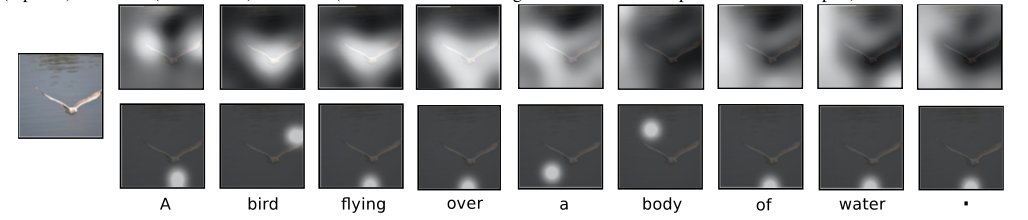
\includegraphics[scale=0.4]{Imgs/show1.png}
\caption{نحوه عمل‌کرد الگوریتم در تغییر نقطه توجه بصری و کلمه تولید شده در هر نقطه. \cite{xu2015show}}
\label{fig:show1}
\end{figure}  
  
  در تمام تصاویر، محدوده‌های روشن‌تر، محدوده‌هایی هستند که در آن‌ها ضریب میانگین‌گیری بیشتر بوده و توجه بیشتری در محاسبات روی آن‌ها متمرکز شده است. شکل \ref{fig:show2} چند نمونه از تصاویر را نمایش می‌دهد که در آن‌ها توجه بصری روی یک جسم منجر به تولید کلمه دقیق متناظر آن جسم شده است. کلمه تولید شده در شرح نهایی تولید شده برای تصویر در زیر هر تصویر نمایش داده شده است.

\begin{figure}[h]
\centering
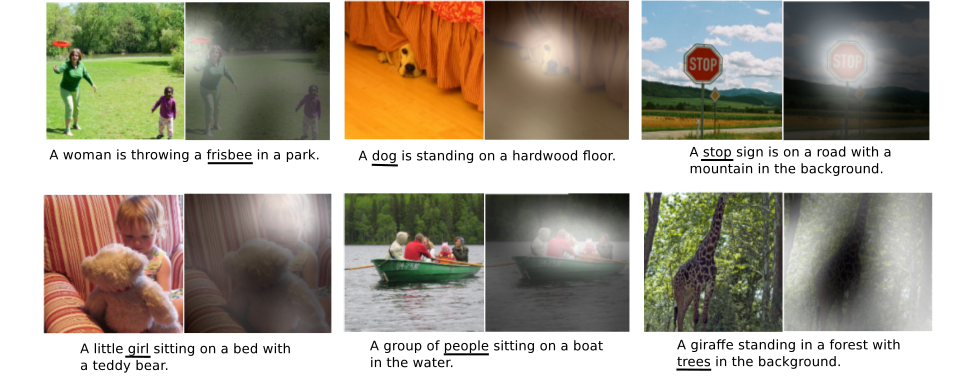
\includegraphics[scale=0.5]{Imgs/show2.png}
\caption{چند نمونه از تصاویر که در آن‌ها توجه بصری روی یک جسم منجر به تولید کلمه دقیق متناظر شده است\cite{xu2015show}. }
\label{fig:show2}
\end{figure}

  به علاوه، شکل \ref{fig:show3} نمایش‌دهنده شرایطی است که در آن کلمه تولید شده متناظر نقطه توجه بصری نیست. با استفاده از بصری‌سازی محل نقطه توجه و کلمه تولید شده در هر مرحله، می‌توان به راحتی مشاهده کرد که کلمه تولید شده متناظر کدام نقطه از تصویر،‌ نامناسب است.
  
  \begin{figure}[h]
  \centering
  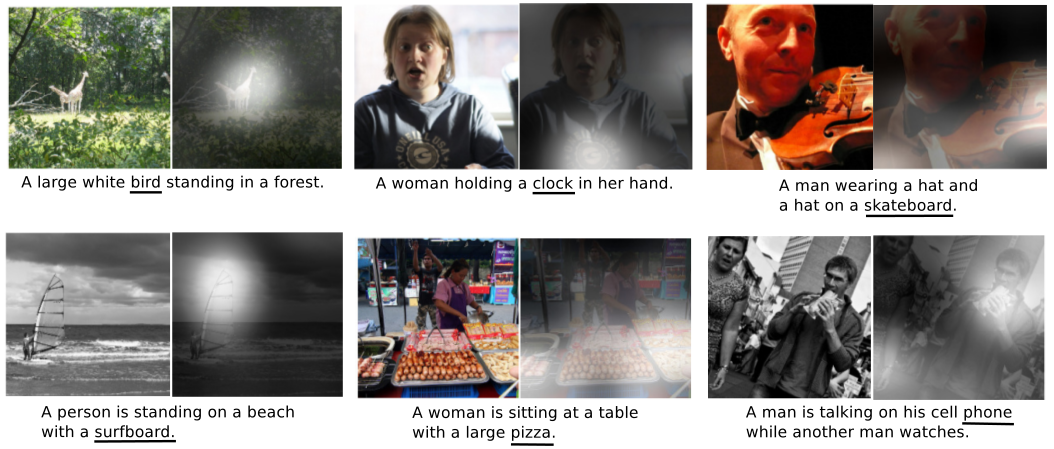
\includegraphics[scale=0.4]{Imgs/show3.png}
  \caption{نمونه‌هایی از تولید کلمات نامناسب مطابق با نقاط توجه استفاده شده در مدل‌\cite{xu2015show}}
  \label{fig:show3}
  \end{figure}
    
علاوه بر موارد فوق، نمونه‌ای از بررسی تمام مراحل تولید شرح متناظر صحنه برای یک تصویر را در حالت‌های استفاده از توجه بصری سخت در شکل \ref{fig:show4} و توجه بصری نرم در شکل \ref{fig:show5} قابل مشاهده است. هر کلمه تولید شده در هر مرحله در کنار میزان فعال‌سازی شبکه مربوط به آن کلمه نمایش داده شده است.

\begin{figure}[h]
\centering 
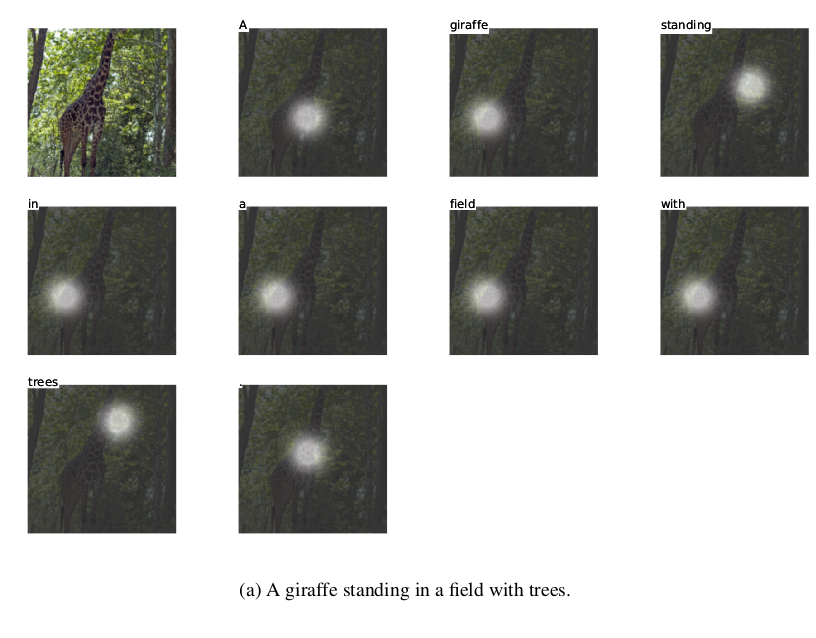
\includegraphics[scale=0.5]{Imgs/show4.png}
\caption{فرایند تولید شرح متناظر تصویر با استفاده از توجه بصری سخت \cite{xu2015show}}
\label{fig:show4}
\end{figure}


\begin{figure}[h]
\centering 
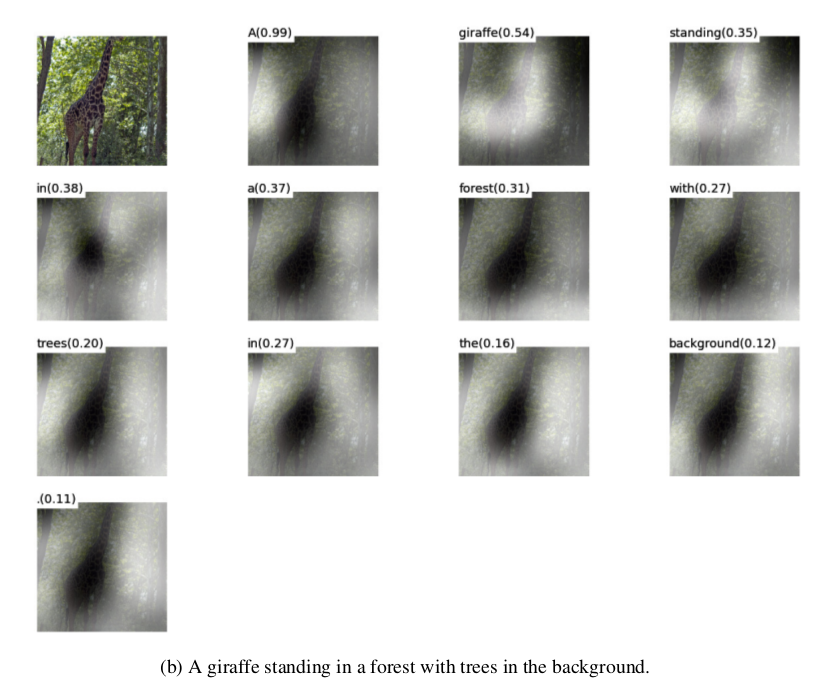
\includegraphics[scale=0.5]{Imgs/show5.png}
\caption{فرایند تولید شرح متناظر تصویر با استفاده از توجه بصری نرم \cite{xu2015show}}
\label{fig:show5}
\end{figure}

